\begin{figure}[htbp]

\centering
\begin{subfigure}[t]{0.49\textwidth}
\captionsetup{labelformat=empty}

\caption{\textbf{AAPL}}
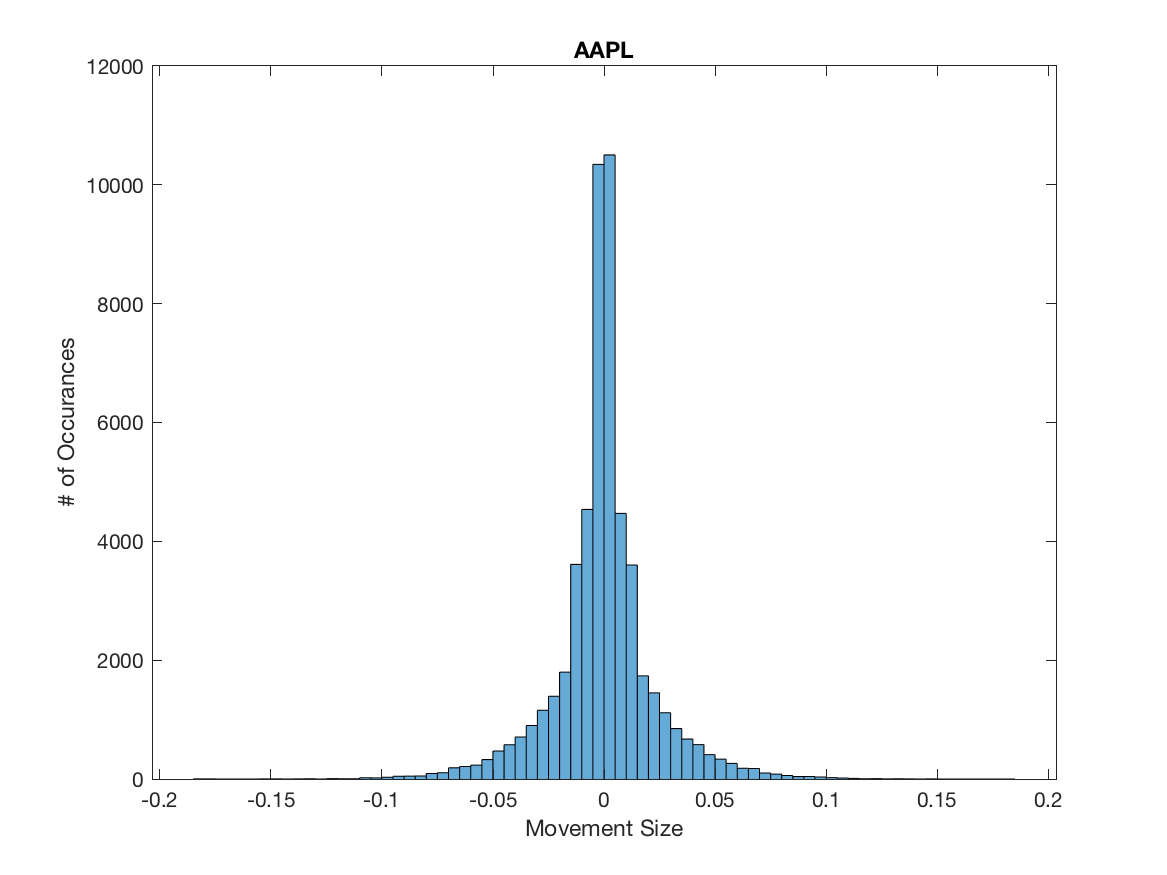
\includegraphics[width=\textwidth, trim = 0 0 0 30, clip]{Tick_Histograms/AAPL_TickHist.png}

\end{subfigure}
\begin{subfigure}[t]{0.49\textwidth}
\captionsetup{labelformat=empty}

\caption{\textbf{AMZN}}
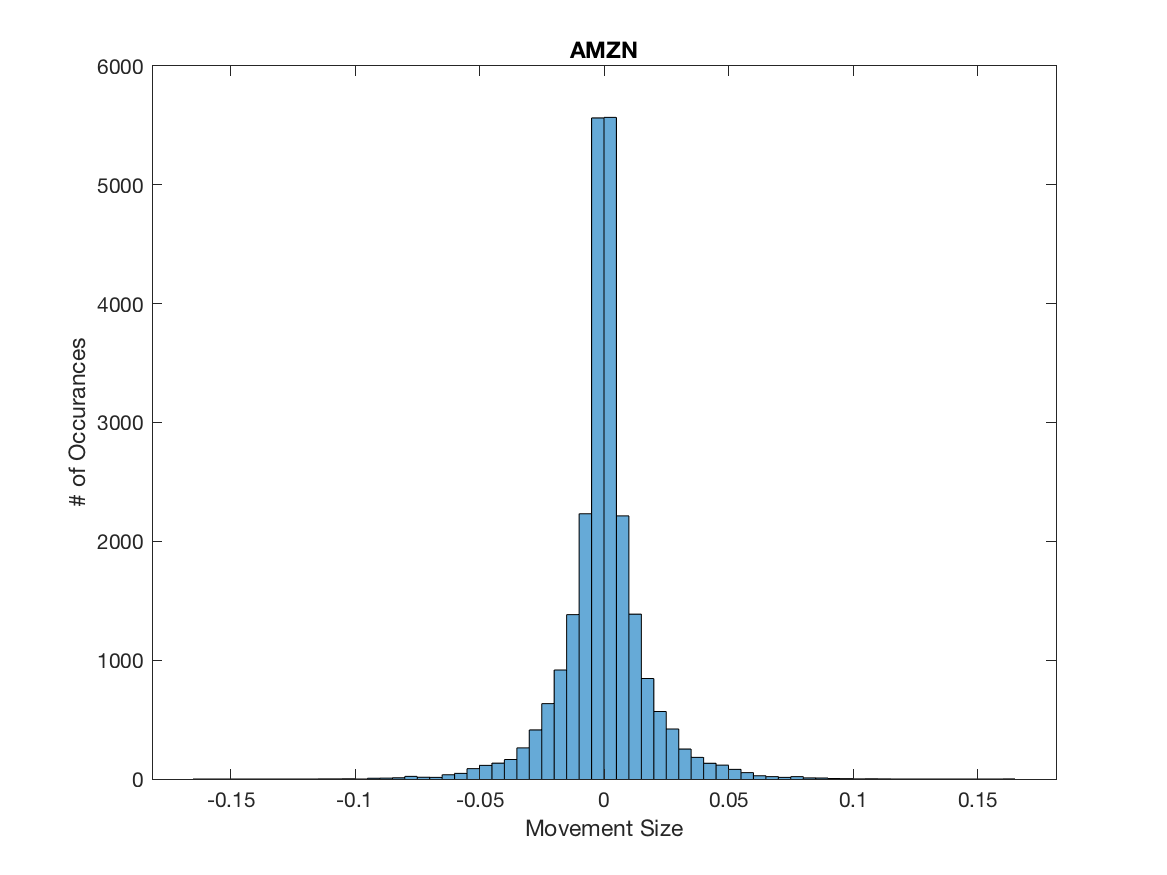
\includegraphics[width=\textwidth, trim = 0 0 0 30, clip]{Tick_Histograms/AMZN_TickHist.png}

\end{subfigure}

\begin{subfigure}[t]{0.49\textwidth}
\captionsetup{labelformat=empty}

\caption{\textbf{GOOG}}
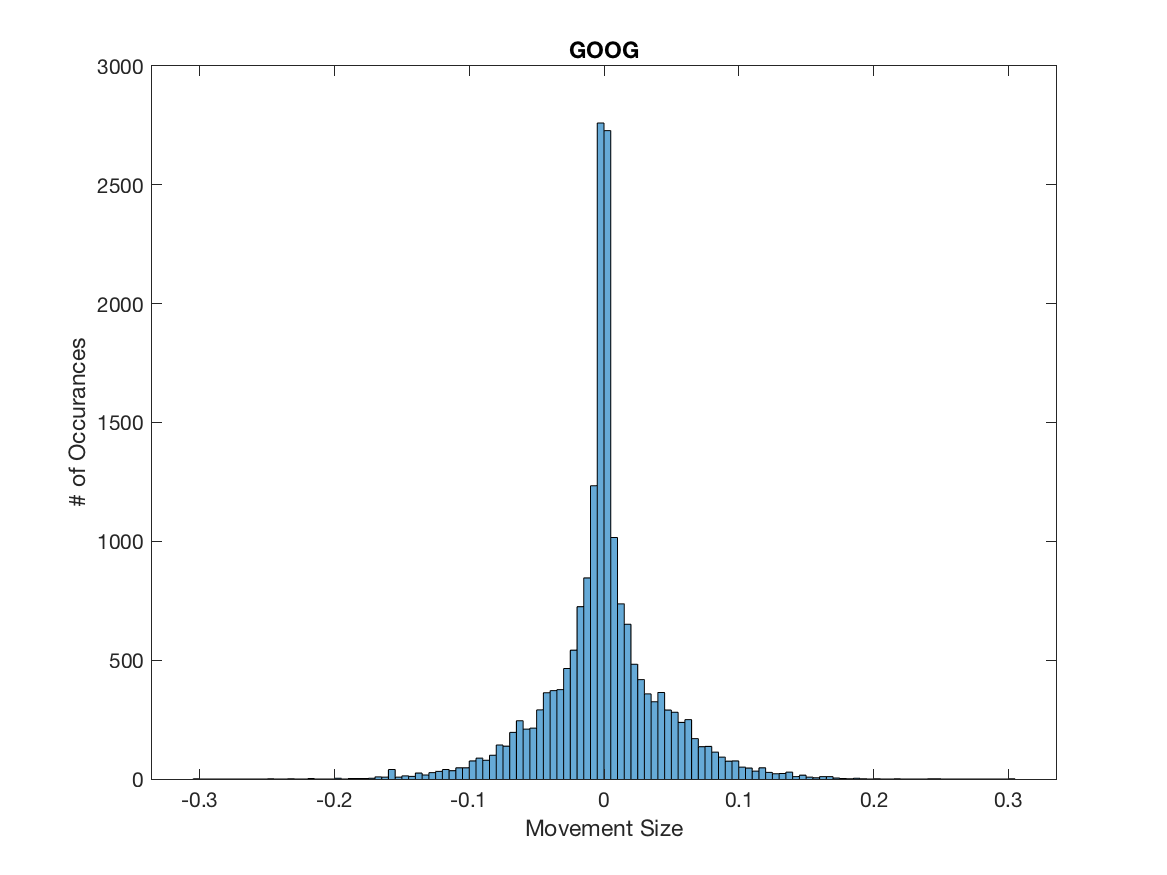
\includegraphics[width=\textwidth, trim = 0 0 0 30, clip]{Tick_Histograms/GOOG_TickHist.png}

\end{subfigure}

\caption{\label{fig:tickhist} We can see clearly that the change in the mid price is often larger than a half tick. These mid price changes make up a significant portion of the actual data, contradicting the assumption needed for the previous model that the mid price changes occur on average at a half tick size.}
\end{figure}